\providecommand{\additionalOptionsForClass}{}
\documentclass[
  accentcolor=tud1c,	% Color theme for TUD corporate design
  colorbacktitle,		% Titlepage has colored background for title area
  inverttitle,			% Font color of title on titlepage is inverted
  \additionalOptionsForClass
  %german%,
  %twoside
]{tudexercise}

\parindent1em
%\parskip2ex

\usepackage[ngerman]{babel}
\usepackage[utf8]{inputenc}
\usepackage{listings}
\usepackage{booktabs}
\usepackage{amsmath}
\usepackage{algorithm2e}
\usepackage{hyperref}
\usepackage{xspace}
\usepackage{tabularx}
\usepackage{tikz}
\usepackage{cleveref}
\usepackage{numprint}
\usepackage{paralist}
\usepackage{verbatim}
\usepackage{tocloft} % for manipulating the table of contents

\usetikzlibrary{shapes}
\usetikzlibrary{calc}
\usetikzlibrary{arrows}
\usetikzlibrary{decorations}

\usepackage{pifont}
\newcommand{\cmark}{\ding{51}\xspace}%
\newcommand{\xmark}{\ding{55}\xspace}%

\usepackage{todonotes}
%\usepackage[disable]{todonotes} % Use this line to hide all todos

\definecolor{commentgreen}{RGB}{50,127,50}
\lstloadlanguages{C++,[gnu]make}
\lstset{language=C++}
\lstset{captionpos=b}
\lstset{tabsize=3}
\lstset{breaklines=true}
\lstset{basicstyle=\ttfamily}
\lstset{columns=flexible}
\lstset{keywordstyle=\color{purple}}
\lstset{stringstyle=\color{blue}}
\lstset{commentstyle=\color{commentgreen}}
\lstset{otherkeywords=\#include}
\lstset{showstringspaces=false}
\lstset{keepspaces=true}
\lstset{xleftmargin=1cm}
\lstset{literate=%
	{Ö}{{\"O}}1
	{Ä}{{\"A}}1
	{Ü}{{\"U}}1
	{ß}{{\ss}}2
	{ü}{{\"u}}1
	{ä}{{\"a}}1
	{ö}{{\"o}}1
	{'}{{\textquotesingle}}1
}

\lstnewenvironment{lstmake} %
{\lstset{language=[gnu]make}} %
{}


\newcommand{\superscript}[1]{\ensuremath{^{\textrm{#1}}}}
\newcommand{\subscript}[1]{\ensuremath{_{\textrm{#1}}}}

\newcommand{\setHeader}[1]{
\providecommand{\examheadertitle}{TODO: Titel einbinden}
\renewcommand{\examheadertitle}{#1}
\begin{examheader}
    \examheadertitle
\end{examheader}
}

\newcommand{\hints}[1]{
\paragraph*{Hinweise}
	\begin{itemize}
		\setlength{\itemsep}{0pt}
		#1
	\end{itemize}
}

\newcommand{\optional}{\xspace(optional)}
\newcommand{\experimental}{\xspace(experimentell)}

\usepackage{fancybox}
\newcommand{\optionaltextbox}{
	\bigskip
	\begin{center}
		\ovalbox{\parbox{0.98\textwidth}{Die Klausur kann ohne diese Aufgabe bestanden werden. Wir empfehlen aber sie trotzdem zu bearbeiten.}}
	\end{center}
}
\newcommand{\experimentaltextbox}{
	\bigskip
	\begin{center}
		\ovalbox{\parbox{0.98\textwidth}{Diese Aufgabe wurde neu erstellt und kann noch Fehler und Inkonsistenzen enthalten. Falls euch etwas derartiges auffällt sprecht uns bitte darauf an oder stellt es auf GitHub in den Issuetracker unter \url{https://github.com/Echtzeitsysteme/tud-cpp-exercises/issues}}}
	\end{center}
}

\newcommand{\enquote}[1]{\glqq#1\grqq\xspace}
\newcommand{\filename}[1]{\texttt{#1}}

\newcommand{\RK}[1]{\todo[]{\textbf{RK:} #1}}
\newcommand{\RKi}[1]{\todo[inline]{\textbf{RK:} #1}}

\newcommand{\ExercisePrefix}[1]{$[$#1$]$ \xspace}
\newcommand{\ExercisePrefixBasics}{\ExercisePrefix{G}}
\newcommand{\ExercisePrefixMemory}{\ExercisePrefix{S}}
\newcommand{\ExercisePrefixObjectOrientation}{\ExercisePrefix{O}}
\newcommand{\ExercisePrefixAdvanced}{\ExercisePrefix{F}}
\newcommand{\ExercisePrefixEmbeddedC}{\ExercisePrefix{C}}
\newcommand{\ExercisePrefixElevator}{\ExercisePrefix{A}}
\newcommand{\ExercisePrefixAdditionalInformation}{\ExercisePrefix{Z}}

\newcommand{\exday}{5}
\cppSetTitle
\setcounter{section}{-1}

\begin{document}

% header and title
\cppSetHeaderAndMakeTitle

\section*{Musterlösungs-/Microcontroller-Projekte in CodeLite importieren}

Die angebotenen Musterlösungs-/Microcontroller-Projekte basieren auf Makefiles.
Daher ist es wichtig, dass du sie entsprechend importierst: \textbf{Workspace -> Add an existing project} und dann zur entsprechenden \filename{.project}-Datei navigieren.


% problems
\section*{Einführung}
Von der Toolseite aus unterscheidet sich die Entwicklung für den Mikrocontroller kaum von den bisherigen Übungen.
Der Aufruf der Toolchain (Compiler, Linker und Flashprogramm) für die Embedded-Entwicklung ist in einem Makefile integriert, das in Eclipse durch den Buildprozess automatisch aufgerufen wird.

Verwende für jede Aufgabe das zugehörige Vorlageprojekt aus dem Übungsrepository (\url{https://github.com/Echtzeitsysteme/tud-cpp-exercises}), da diese sowohl das Makefile, als auch notwendige Bibliotheken im Ordner \texttt{uc\_includes} zur Verwendung des Boards enthalten.

\hints{
	\item Sollte der Flashvorgang fehlschlagen, kann es helfen den Schiebeschalter auf dem Board auf \textbf{PROG} zu schalten.
	Nach dem Flashvorgang setzt man dann den Schiebeschalter auf \textbf{RUN} und startet das Programm mit Hilfe der blauen Resettaste.
	\item Pool-PCs: Das USB-Kabel muss am Hub in der Buchse stecken, die mit \emph{Data} beschriftet ist.
	\item Variablen dürfen in dieser Übung im Gegensatz zu C++ nur am Anfang eines Anweisungsblocks deklariert werden.
	Erst ab dem C99 Standard (welche hier nicht verwendet wird) dürfen Deklarationen an beliebigen Stellen erfolgen.
}

\section{Test}
Teste das Zusammenspiel von Eclipse, Compiler und Flashvorgang auf dem Mikrocontroller, indem du das vorgegebene Projekt zu dieser Aufgabe baust.
Auf der Siebensegmentanzeige des Boards sollte im Erfolgsfall eine 42 erscheinen.



\section{Siebensegmentanzeige}
\label{exercise7Segment}

Implementiere ein Programm, das die Zahlen 0 bis 99 auf der Siebensegmentanzeige ausgibt.
Nach jeder Ausgabe einer Zahl soll eine Pause eingelegt werden.

\begin{center}
	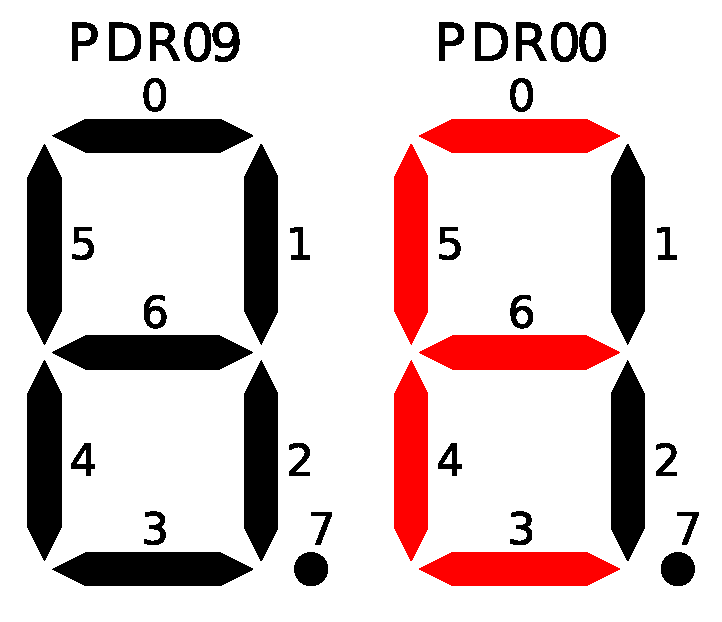
\includegraphics[width=0.2\textwidth]{figures/7seg_e}
\end{center}

Für die Ausgabe der Zahlen 0 bis 9 steht dir das Array \texttt{DEC7SEG} zur Verfügung, welches die benötigten Werte für die jeweiligen Ziffern enthält.
Die beiden Anzeigen sind an den Ports 09 und 00 angeschlossen.
Die Ansteuerung erfolgt logisch invertiert, das bedeutet, dass ein Segment bei einer logischen 0 leuchtet und umgekehrt.
Beispiel: Ein \glqq{}E\grqq{} kann durch das Setzen der Pins 0, 3, 4, 5 und 6 (Binär: 10000110, bzw. Hexadezimal: 0x86) auf low gezeichnet werden.

\begin{lstlisting}
	long d;					// always define variables at the beginning of a block!
	for (d = 0; d < DELAY; ++d) {
		__wait_nop();		// wait one cycle
	}
\end{lstlisting}

Die Pause kann durch eine Schleife produziert werden, die in jedem Zyklus den Befehl \texttt{\_\_wait\_nop()} aufruft.
Eine Konstante \texttt{DELAY} steht dir für die Anzahl der Schleifendurchläufe zur Verfügung.
Achte insbesondere darauf, dass du für die Schleifenzählervariable den Datentyp \texttt{long} verwendst.



\section{Buttons}
Implementiere einen Counter der bei 00 startet und bis 99 zählen kann.
Bei Druck auf die rechte Taste soll der Wert erhöht, bei Druck auf die linke Taste verringert werden.
Nutze die Siebensegmentanzeige aus der vorherigen Aufgabe zur Anzeige des aktuellen Wertes.

Wird 99 angezeigt und die rechte Taste gedrückt, soll der Counter auf 00 gesetzt werden.
Umgekehrt gilt: Falls der Counter 00 anzeigt und die linke Taste gedrückt wird, soll er auf 99 umspringen.

Der linke Taster ist an Port 07 Pin 0, der rechte an Port 07 Pin 1 angeschlossen.
Bei gedrücktem Taster liegt ein Low-Pegel am Eingang, sonst ein High-Pegel.
Du kannst den Zustand eines Pins wie folgt abfragen:
\begin{lstlisting}
char leftButton, rightButton;
leftButton = PDR07_P0; 
rightButton = PDR07_P1;
\end{lstlisting}

\hints{
	\item Ein Button ist üblicherweise für mehrere tausend CPU-Zyklen gedrückt.
	\item Ein Tastendruck ist durch den Übergang von \emph{high} auf \emph{low} definiert.
	Da in jedem Zyklus nur der aktuelle Wert abgefragt werden kann, musst du den aktuellen Wert mit einem gespeicherten Wert aus dem vorigen Durchlauf vergleichen.
	\item Die Moduloberechnung von negativen Zahlen kann problematisch sein.
	Hier hilft es, wenn du vor der Modulo\-operation den Divisor hinzuaddierst.
}



\section{Hilfsfunktionen}
\label{exercise7SegmentUtil}
Implementiere wie in \ref{exercise7Segment} einen Zähler von 0 bis 99, jedoch unter Verwendung von eigens dafür geschriebenen Hilfsfunktionen:
\begin{lstlisting}
void wait(long w)				// wait for w cycles
void setLeft7Seg(int i)		// set left display to the given number i (if 0 <= i <= 9)
void setRight7Seg(int i)	// set right display to the given number i (if 0 <= i <= 9)
void set7Seg(int i)			// set the seven-segment display to the given number
\end{lstlisting}



\section{A/D-Wandler}
Schreibe ein Programm, das den Spannungswert von \emph{AN1} (linker Schieberegler) auf der linken Siebensegmentanzeige und den Spannungswert von \emph{AN2} (rechter Schieberegler) auf der rechten Siebensegmentanzeige ausgibt.
Skaliere dazu den resultierenden Wertebereich (0 bis 255) auf 0 bis 9.

Mache dich mit folgenden Funktionen vertraut und verwende sie zur Initialisierung und anschließender Verwendung des A/D-Wandlers:
\begin{lstlisting}
void initADC(void)				// initialize the ADCs
int getADCValue(int channel)	// read the value from channel 1 or 2
\end{lstlisting}

\hints{
	\item Einige Funktionen aus \ref{exercise7SegmentUtil} kannst du hier wiederverwenden.
	\item Der Wert für \texttt{ADSR} besteht aus 16 Bits (0110 11xx xxxy yyyy\textsubscript{b}), wobei xxxxx für den Startkanal der Konvertierung und yyyyy für den Endkanal steht.
	Für unsere Zwecke nehmen diese beiden 5\,Bit Blöcke immer entweder 00001\textsubscript{b} = 1 (AN1) oder 00010\textsubscript{b} = 2 (AN2) an.
	Daher lässt sich der \texttt{ADSR} auch wie folgt über einen binären Shift und zwei Addition bestimmen:
	$$\texttt{ADSR} = 0110110000000000\textsubscript{b} + (xxxxx\textsubscript{b} << 5) + yyyyy\textsubscript{b} = 0x6c00 + (x << 5) + y$$
}



\section*{Einführung LCD}
Die Ansteuerung des LCD erfolgt über Pins mit festgelegten Funktionen.
Zur Vereinfachung wurden bereits im Projekt für diese Aufgabe Definitionen vorgegeben, sodass die Pins über einfache Namen angesteuert werden können. Die Namen entsprechen den Pins, wie sie im Datenblatt (\url{https://github.com/Echtzeitsysteme/tud-cpp-exercises/blob/master/doc/Display_AV128641YFBY-WSV.pdf}) ab Seite 10 zu finden sind.

\begin{center}
	\begin{tabular}{l|l|l}
		\toprule
		\textbf{Name} & \textbf{Funktion} & \textbf{Pin/Port} \\ 
		\midrule
		LCD\_PORT\_DB & Datenbus (DB0 - DB7) & P01 \\ 
		LCD\_PIN\_DI & Data (1) / Instruction (0) & P02\_0 \\ 
		LCD\_PIN\_RW & Read (1) / Write (0) & P02\_1 \\ 
		LCD\_PIN\_E & Enable & P02\_2 \\ 
		LCD\_PIN\_CS1 & Linker Chip (1 = aktiv) & P02\_3 \\ 
		LCD\_PIN\_CS2 & Rechter Chip (1 = aktiv) & P02\_4 \\ 
		LCD\_PIN\_RESET & Reset-Signal (0 = aktiv) & P02\_5 \\ 
		\bottomrule
	\end{tabular}
\end{center}

\paragraph{Display einschalten}

Das Display muss vor der Benutzung eingeschaltet werden:
\begin{lstlisting}
// Display on
LCD_PORT_DB = 0x3F; 
// Display off
LCD_PORT_DB = 0x3E; 
\end{lstlisting}

\paragraph{Displayhälften (Chip-Select Signal)}
Das Display ist logisch aufgeteilt in zwei Hälften zu je 64 x 64 Pixel (siehe untenstehende Grafik, MSB/LSB = Most/Least Significant Bit).
\begin{center}
	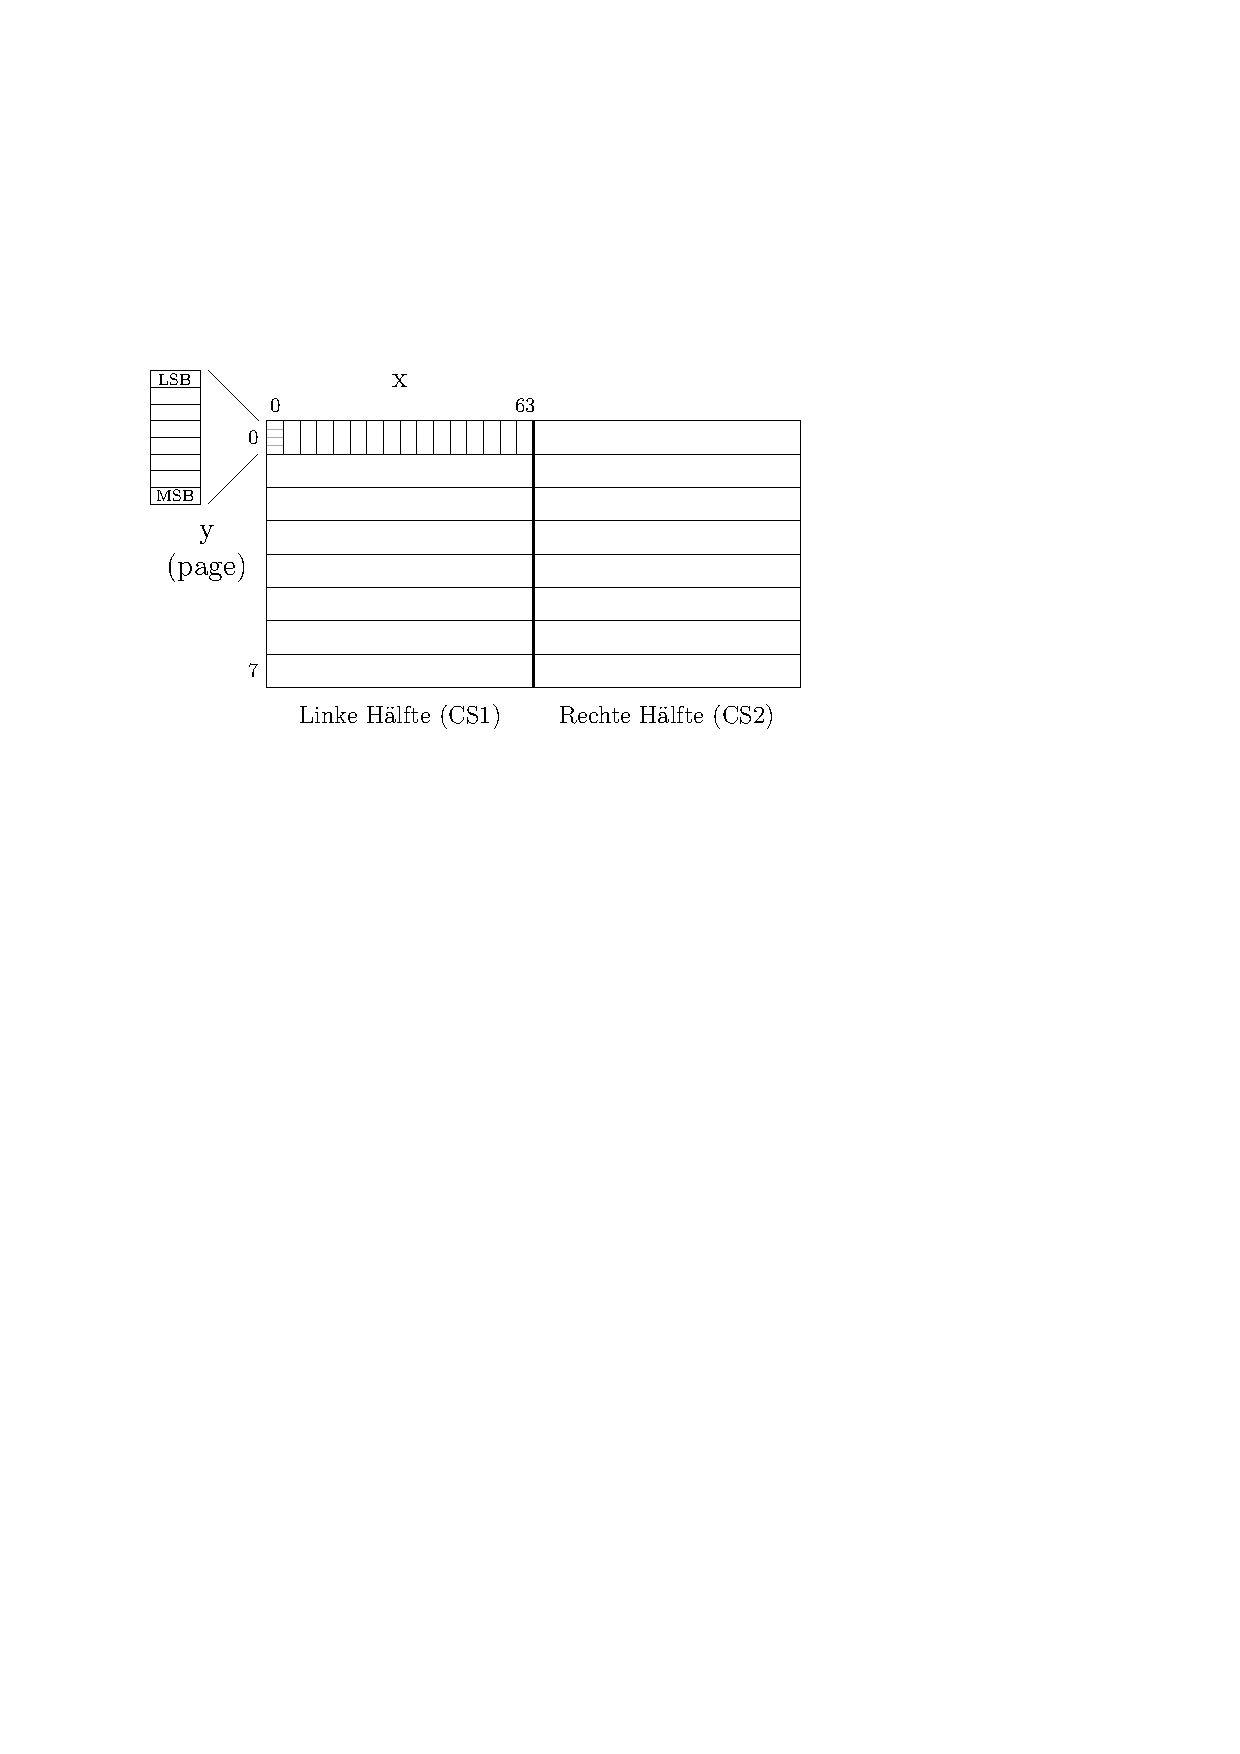
\includegraphics[width=0.6\textwidth]{figures/display_aufbau}
\end{center}

Welche Hälfte einen Befehl verarbeiten soll, wird ausgewählt, indem deren Chip-Select-Signal auf 1 gesetzt wird, das andere auf 0:
\begin{lstlisting}
// select left display part (CS1)
LCD_PIN_CS1 = 1;
LCD_PIN_CS2 = 0;
// select right display part (CS2)
LCD_PIN_CS1 = 0;
LCD_PIN_CS2 = 1;
\end{lstlisting}

\subsection*{Befehle senden}
Ein Befehl an das Display besteht grundsätzlich aus zwei Phasen:
\begin{enumerate}
\item
Setzen der entsprechenden Pins (meist \texttt{LCD\_PIN\_DI}, \texttt{LCD\_PORT\_DB}).

Eventuell selektieren der Displayhälfte über \texttt{LCD\_PIN\_CS1, LCD\_PIN\_CS2}.

\item
Senden des \texttt{enable}-Signals.
Setze dazu den Enable-Pin auf 1, warte kurz, setze den Pin wieder auf 0 und warte erneut kurz.
Verwende als Warteintervall die Konstante \texttt{LCD\_T}.

Es empfiehlt sich, für dieses Signal eine eigene Funtkion zu schreiben (\texttt{void lcd\_sendEnable(void)}).
\end{enumerate}

\subsection*{Auf das Display zeichnen}

Das Vorgehen zum Zeichnen sieht in etwa wie folgt aus:
\begin{enumerate}
	\item Setzen der x-Adresse (Zeile)
	\item Setzen der y-Adresse (Spalte)
	\item Senden von 8 Bit Daten (eine \glqq{}Zelle\grqq{} von 8 Pixeln Höhe)
\end{enumerate}



\section{LCD Basics}
Implementiere ein Programm, dass die linke Seite des Displays ansteuert und alle Zellen mit dem Wert AA\textsubscript{h} (10101010\textsubscript{b}) belegt, was einem sehr feinen Streifenmuster entspricht.

Der \texttt{x}-Zähler wird nach dem Senden von Daten zum Display automatisch hochgezählt.
Somit ist es sinnvoll, beim Zeichnen zuerst über die Seiten (\texttt{y}) zu iterieren und innerhalb dieser Schleife über die Spalten (\texttt{x}):
\begin{lstlisting}
char x, y;
for (y = 0; y < 8; ++y) {
	// LCD: set y address to 'y', set x address to 0
	for (x = 0; x < 64; ++x) {
	    // LCD: draw pixel -> column/x address is incremented automatically
	}
}
\end{lstlisting}

\hints{
	\item Denke daran, \texttt{LCD\_PIN\_E} zu Beginn des Programms mit 0 zu initialisieren.
	\item Das Reset-Signal (\texttt{LCD\_PIN\_RESET}) muss immer 1 (deaktiviert) sein.
}



\section{LCD}
Nun soll das Display wie ein Bildschirm angesteuert werden können.
Dazu wirst du einen Framebuffer verwenden, der den Bildschirminhalt repräsentiert.
In jeder Iteration wird der Framebuffer zunächst vollständig vorbereitet und dann am Stück übertragen.

Die Vorlage enthält bereits ein Array \texttt{lcd\_buffer}, das als Framebuffer fungieren soll.

Implementiere folgende Funktionen:
\begin{lstlisting}
void lcd_clear();     // clear the frame buffer, setting all pixels to 0
void lcd_drawPixel(int x, int y, int black);    // set (black == 1) or clear (black == 0) a pixel in the frame buffer, do nothing, if any input parameter is invalid
void lcd_flush();    // display the frame buffer on the LCD
\end{lstlisting}

\hints{
	\item Ein Testprogramm steht bereits zur Verfügung, welches ein Schachbrettmuster auf dem Display ausgibt -- wenn deine Funktionen komplett und korrekt implementiert sind.
	\item Achte auch hier darauf, dass das Display zunächst per Befehl eingeschaltet werden muss (\emph{Display on}).
	\item Für die Funktion \texttt{lcd\_drawPixel} werden die Bitoperationen AND und OR sowie der Shift-Operator benötigt.
	Eine Skizze kann hier sinnvoll sein, um sich vorzustellen, wie die Bitoperationen arbeiten.
	\item Wenn du später bewegte Dinge visualisierst, kann es sein, dass das Display flimmert.
	Hier hilft es, entweder die Anzeige nur zu verändern, wenn sich tatsächlich etwas bewegt oder das Display vor dem Schreiben des Framebuffers aus- (\emph{Display off}) und danach wieder einzuschalten (\emph{Display on}).
}

\end{document}
